To ensure that the fridge is designed and constructed in a logical and efficient way, 
a Gantt chart has been produced showing the expected outcomes as the weeks go by (seen in Figure \ref{fig:gantt}). 
Furthermore, figure \ref{fig:risk_management} shows a list of foreseeable risks compared to the values of a risk matrix. 
By following these two guides, a solid proof of concept will be produced by the final presentation and report deadlines.

\begin{figure}[H]        
    \centering
    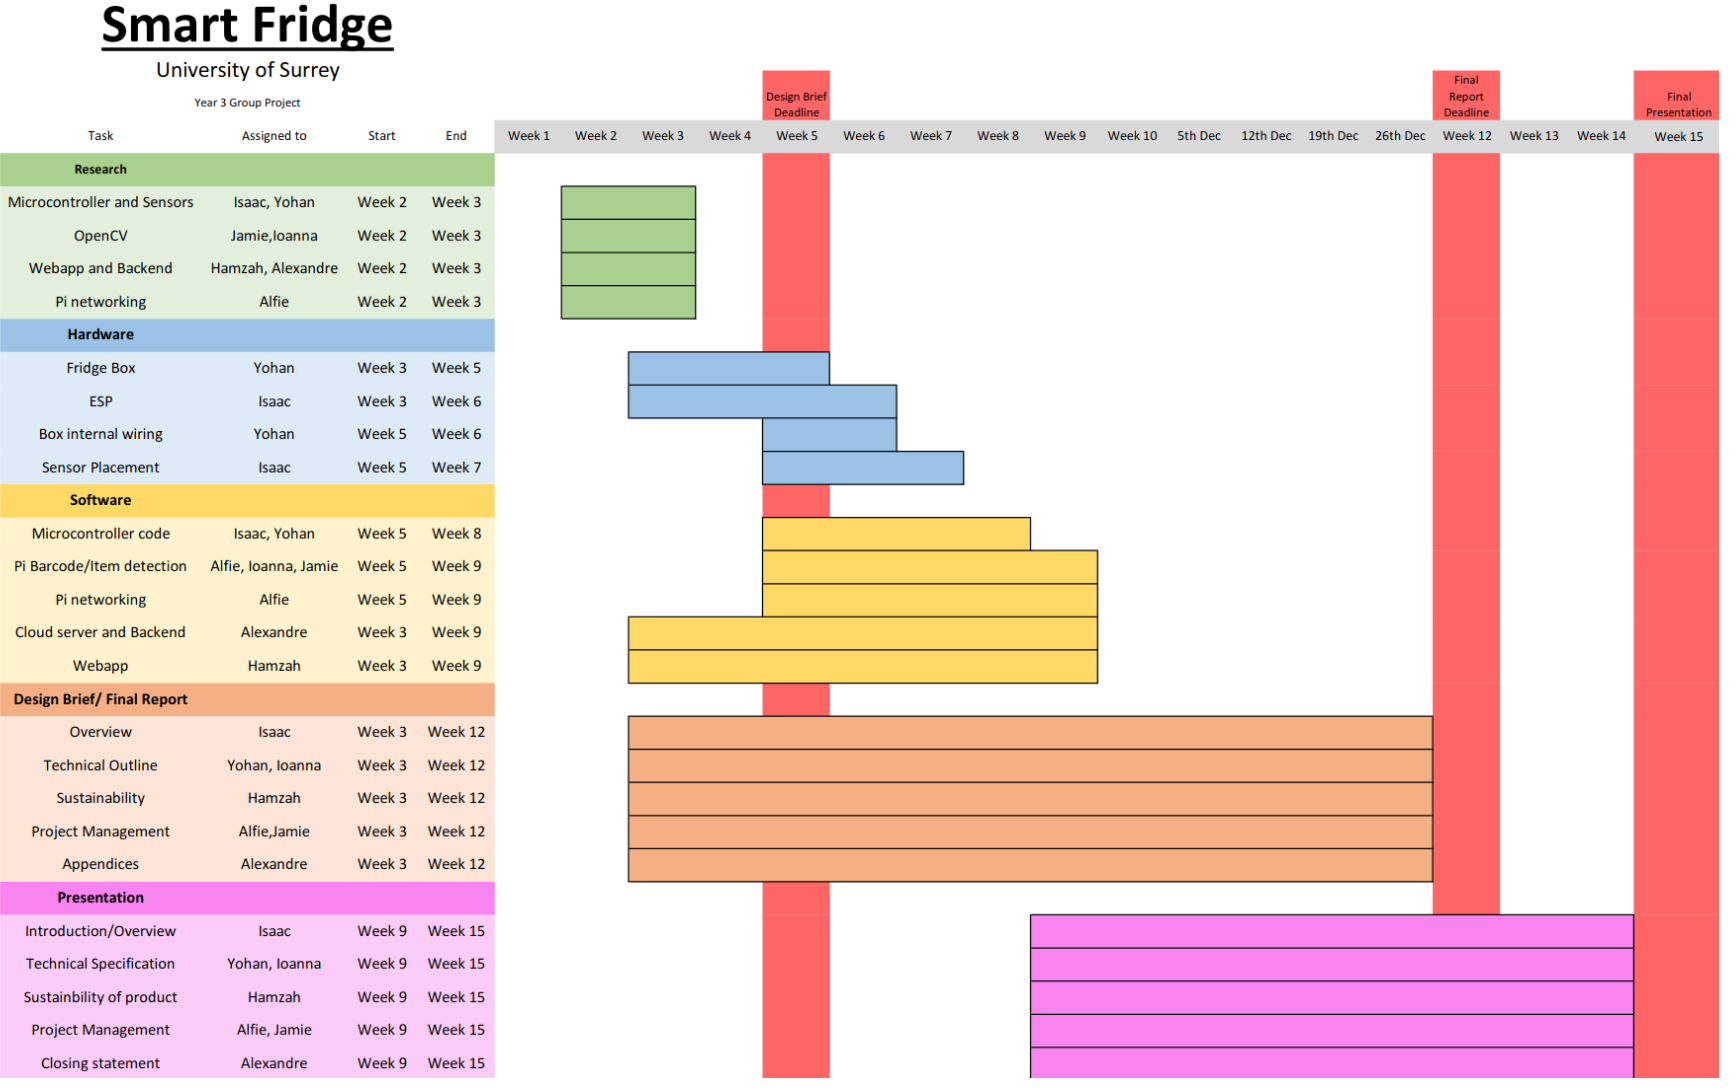
\includegraphics[width=0.66\textwidth]{gantt.png}
    \caption{Gantt Chart}
    \label{fig:gantt}
\end{figure} 

\begin{figure}[H]        
    \centering
    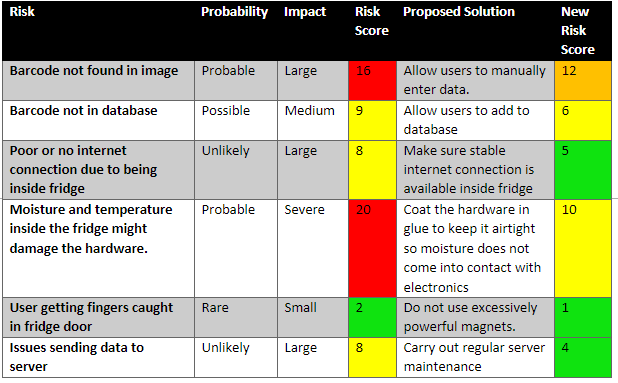
\includegraphics[width=0.66\textwidth]{Risk-Managment.png}
    \caption{Risk Management}
    \label{fig:risk_management}
\end{figure} 

As for costing, the “Fridge” outer shell we require $2m^2$ of acrylic, approximately £30.
ESP32-Cam costs £11, RPi £32 and Weight Sensor £9 [2][3][4]. Smaller components will be provided by the UG Labs. 

\subsection{References}

\begin{enumerate}
    \item https://sdgs.un.org/goals      
    \item https://thepihut.com/products/esp32-camera-module-development-board-ov2640
    \item https://thepihut.com/products/raspberry-pi-3-model-a-plus
    \item https://www.amazon.co.uk/Weight-Sensor-Weighing-Arduino-Raspberry-Black/dp/B07G29TKRH/
\end{enumerate}
